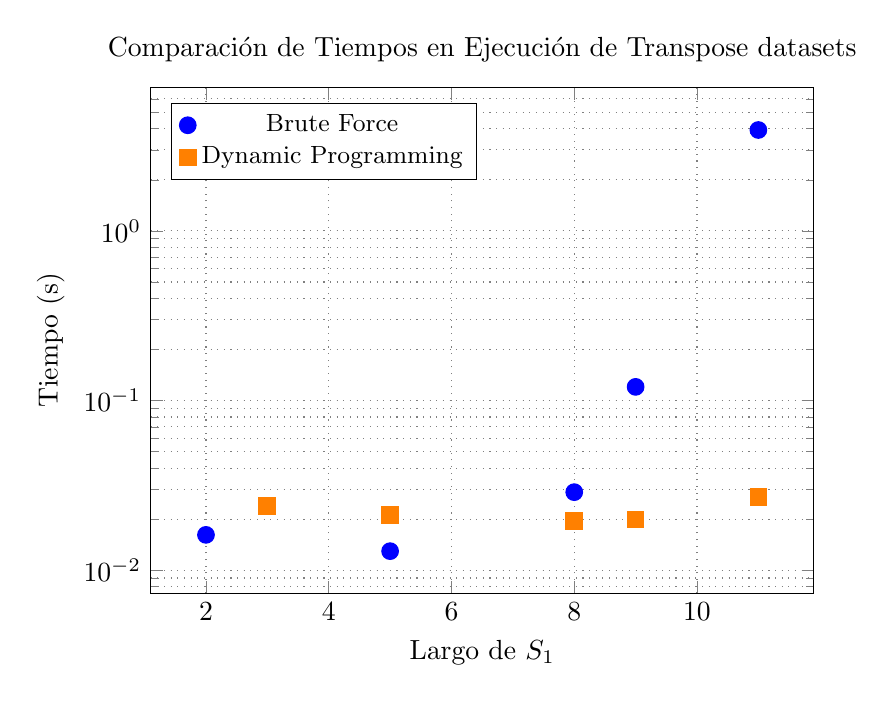
\begin{tikzpicture}
    \begin{axis}[
        ylabel={Tiempo (s)},
        xlabel={Largo de $S_1$},
        title={Comparación de Tiempos en Ejecución de Transpose datasets},
        legend pos=north west,
        ymode=log, % Escala logarítmica para resaltar diferencias de tiempo
        grid=both,
        grid style={dotted, gray},
        legend style={font=\small},
        width=10cm,
        height=8cm
    ]

    % Datos de brute force (color azul)
    \addplot[
        only marks,
        mark=*,
        color=blue,
        mark options={scale=1.5}
    ] coordinates {
        (2, 0.01616)
        (5, 0.012956)
        (8, 0.028852)
        (9, 0.120391)
        (11, 3.93128)
    };
    \addlegendentry{Brute Force}

    % Datos de dynamic programming (color naranja)
    \addplot[
        only marks,
        mark=square*,
        color=orange,
        mark options={scale=1.5}
    ] coordinates {
        (3, 0.024023)
        (5, 0.0211)
        (8, 0.019574)
        (9, 0.019883)
        (11, 0.027025)
    };
    \addlegendentry{Dynamic Programming}

    \end{axis}
\end{tikzpicture}